\documentclass{article}
\usepackage[english]{babel}
\usepackage[letterpaper,top=2cm,bottom=2cm,left=3cm,right=3cm,marginparwidth=1.75cm]{geometry}

% Useful packages
\usepackage{amsmath}
\usepackage{graphicx}
\usepackage[colorlinks=true, allcolors=blue]{hyperref}
\usepackage{xcolor}
\usepackage{algcompatible}
\usepackage{algorithm}
\usepackage[noend]{algpseudocode}
\usepackage{pgffor}
\usepackage{pgfplots}
\usepackage{caption}
\usepackage{float}
\usepackage{nameref}
\usepackage[T1]{fontenc}
\usepackage{lmodern}
\usepackage{authblk}
\usepackage{bm}

\title{\textbf{AMMM Final Project Report}}

%\author{123(\href{mailto:@estudiantat.upc.edu}{Email})
%\and 123(\href{mailto:@estudiantat.upc.edu}{Email})}
\author[1]{Elly Attal}
\author[2]{Jose Arias}

\affil[1]{MIRI \href{mailto:@estudiantat.upc.edu}{elly.attal@estudiantat.upc.edu}}
\affil[2]{MIRI \href{mailto:@estudiantat.upc.edu}{jose.ricardo.arias@estudiantat.upc.edu}}


\begin{document}
\maketitle


\tableofcontents

\newpage

\section{Martian Network Destruction Problem Statement}

The Martian Network Destruction problem can be formally stated as follows:\\
\\
\textbf{\textit{Given}}:
\begin{itemize}
    \item The set $B = \{1, 2, \ldots, n\}$ of Martian military bases. For each pair of bases $i, j \in B$, the number of specialist hours $t_{ij}$ required to destroy the pipe between them is specified (where $t_{ij} < 0$ indicates that no pipe exists between the two bases $i$ and $j$).

    \item The set $S = \{1, 2, \ldots, m\}$ of specialists. For each specialist $k \in S$, the available working hours $w_k$ and the cost per assignment $c_k$ are specified.
\end{itemize}

\textbf{\textit{Find:}}
\begin{itemize}
    \item The destruction of pipes must create a disconnected network (the graph becomes non-connected, preventing fuel from transporting across all bases).

    \item Each specialist can be assigned to at most one pipe.

    \item Each pipe we want to destroy must receive enough specialist hours to reach its destruction requirement $t_{ij}$.
\end{itemize}

\textbf{\textit{Objective}}:
\begin{itemize}
    \item Minimize the total cost of specialist assignments to disconnect the network.
\end{itemize}


\section{ILP Model Formulation}

This problem can be modeled as an Integer Linear Program. To achieve this, the following sets and parameters are defined:\\
\\
\textit{B} \hspace{1.3cm} Set of n bases, index i, j. \\
\textit{S} \hspace{1.3cm} Set of m specialists, index s. \\
\textit{E} \hspace{1.3cm} Set of edges (pipelines) between bases. \\
\textit{$w_s$} \hspace{1.15cm} Number of working hours of specialist s. \\
\textit{$c_s$} \hspace{1.25cm} Cost of using specialist s. \\
\textit{$t_{ij}$} \hspace{1.25cm} Hours required to destroy the pipeline between bases i and j. \\
\\
The following decision variables are also defined:\\
\\
\textit{$x_{se}$} \hspace{1.15cm} Binary. Equal to 1 if specialist s is assigned to edge e; 0 otherwise. \\
\textit{$d_e$} \hspace{1.25cm} Binary. Equal to 1 if edge (pipeline) e is destroyed; 0 otherwise. \\
\textit{$g_i$} \hspace{1.3cm} Binary. Equal to 1 if base i belongs to group 1; 0 if it belongs to group 0. \\
\\
Finally, the ILP model for the pipe destruction problem is as follows:
\begin{equation}
    \textrm{minimize} \quad \sum_{s \in S} \sum_{e \in E} c_s \cdot x_{se}
\end{equation}
subject to:
\begin{equation}
    \sum_{e \in E} x_{se} \leq 1 \qquad \forall s \in S
\end{equation}
\begin{equation}
    \sum_{s \in S} w_s \cdot x_{se} \geq t_{ij} \cdot d_e \qquad \forall e = (i,j) \in E
\end{equation}
\begin{equation}
    x_{se} \leq d_e \qquad \forall s \in S, \forall e \in E
\end{equation}
\begin{equation}
    d_e \geq g_i - g_j \qquad \forall e = (i,j) \in E
\end{equation}
\begin{equation}
    d_e \geq g_j - g_i \qquad \forall e = (i,j) \in E
\end{equation}
\begin{equation}
    1 \leq \sum_{i \in B} g_i \leq n-1
\end{equation}
\\


\section{Heuristics Method}

\subsection{Greedy Method}

\subsubsection{Variable Declaration}

\textbf{Phase 1: Minimum Cut Variables}
\begin{itemize}
    \item $Bases$: Set of bases in the network.
    \item $Pipes$: Set of all pipes connecting bases.
    \item $Demand_p$: The demand (flow requirement) for pipe $p$.
    \item $Partition$: Binary assignment of bases to groups $\{0, 1\}$. Equal to 0 if base $i$ belongs to group 0, 1 otherwise.
    \item $CutPipes$: Set of pipes crossing the partition, i.e., pipes $p = \langle i,j \rangle$ where $Partition[i] \neq Partition[j]$.
\end{itemize}

\textbf{Phase 2: Specialist Assignment Variables}
\begin{itemize}
    \item $Specialists$: Set of available specialists.
    \item $Capacity_s$: The capacity (work units) that specialist $s$ can provide.
    \item $Cost_s$: The cost of hiring specialist $s$.
    \item $CostEffectiveness_s$: Ratio $Cost_s / Capacity_s$ for specialist $s$.
    \item $Solution$: Set of assignments $\langle s, p \rangle$. Each specialist can be assigned to at most one pipe.
    \item $AssignedSpecialists$: Set of specialists currently assigned in the $Solution$.
    \item $RemainingDemand_p$: Uncovered demand for pipe $p$ after current assignments.
\end{itemize}

\subsubsection{Greedy Cost Function}

Our greedy approach operates in two sequential phases:
\\[0.2cm]

\textbf{Phase 1: Minimum Cut Computation}
\\[0.2cm]
We found two greedy algorithms to find the minimum cut partition of the network:

\begin{enumerate}
    \item \textbf{Karger's Algorithm} (randomized): Repeatedly contracts random edges weighted by demand until two super-nodes remain. The original algorithm runs multiple iterations to increase the probability of finding the true minimum cut.

    \item \textbf{Stoer-Wagner Algorithm} (deterministic): Uses maximum adjacency ordering to systematically find the global minimum cut through a series of min-cut phases.
    This algorithm is better for dense graphs.
    \\[0.2cm]
    The choice of the algorithm can be made in config.dat with minCut.
\end{enumerate}

Both algorithms minimize the total demand in terms of hours crossing the partition:

\begin{equation}
\text{MinCut} = \min_{\text{Partition}} \sum_{p \in \text{Pipes}} \text{Demand}_p \times \mathbf{1}[\text{Partition}[\text{base}_i(p)] \neq \text{Partition}[\text{base}_j(p)]]
\end{equation}

The output is a binary partition that defines which pipes must be covered by specialists (the $CutPipes$).
\\[0.5cm]

We decided to select Karger's algorithm with \textbf{only one} iteration per Greedy exploration, so we obtain a randomized cut that introduces diversification, which is particularly valuable when the true minimum cut is infeasible.
\\[0.5cm]

\textbf{Phase 2: Greedy Specialist Assignment}
\\[0.2cm]
For the set of $CutPipes$ identified in \textbf{Phase 1}, we iteratively assign specialists using a greedy cost-effectiveness criterion:

\begin{displaymath}
    q(\langle s, p \rangle, \text{Solution}) = \begin{cases}
    \text{CostEffectiveness}_s & \text{if assigning } s \text{ to } p \text{ is feasible}\\
    +\infty & \text{otherwise}
    \end{cases}
\end{displaymath}

We always select the specialist-pipe pair with the \textbf{lowest cost-effectiveness} (most efficient specialist) among those that:
\begin{enumerate}
    \item Have not been assigned yet
    \item Can contribute to covering the remaining demand of pipe $p$
\end{enumerate}

The assignment continues until all pipes in $CutPipes$ are fully covered or the problem becomes infeasible.

\subsubsection{Pseudocode}

\begin{algorithm}[H]
\renewcommand{\thealgorithm}{}
\caption{Greedy Algorithm}
\begin{algorithmic}
\Statex
\Statex \textbf{PHASE 1: MINIMUM CUT}
\Function{ComputeMinCut}{$Bases$, $Pipes$}
\If{$minCutAlgorithm = \text{"Karger"}$} \Comment{Karger}
    % \State $iterations \gets \max(10, \lfloor(|Bases|^2 \times \ln(|Bases|)) / 2\rfloor)$
    \State $iterations \gets 1$
    \State $cutWeight, Partition \gets \text{Karger}(Bases, Pipes, iterations)$
\Else \Comment{Stoer-Wagner}
    \State $cutWeight, Partition \gets \text{StoerWagner}(Bases, Pipes)$
\EndIf
\State \textcolor{red}{$CutPipes \gets \{p \in Pipes \mid Partition[base_i(p)] \neq Partition[base_j(p)]\}$}
\State \Return $CutPipes$
\EndFunction
\Statex
\Statex \textbf{PHASE 2: GREEDY SPECIALIST ASSIGNMENT}
\Function{GreedyConstruction}{ }
\State $Solution \gets \phi$
\State $AssignedSpecialists \gets \phi$
\State $CutPipes \gets \text{ComputeMinCut}(Bases, Pipes)$
\Statex
% \State \Comment{Sort pipes by demand (descending) - hardest first}
\State $SortedPipes \gets \text{Sort}(CutPipes, key=Demand, reverse=\text{True})$
\Statex
% \State \Comment{Sort specialists by cost-effectiveness (ascending) - best first}
\State $SortedSpecialists \gets \text{Sort}(Specialists, key=CostEffectiveness)$
\Statex
\For{each $p \in SortedPipes$}
    \State $RemainingDemand_p \gets Demand_p$
    \While{$RemainingDemand_p > 0$}
        \State \Comment{Find best available specialist}
        \State \textcolor{red}{$s \gets \arg\min_{s' \in SortedSpecialists \land s' \notin AssignedSpecialists} CostEffectiveness_{s'}$}
        \If{$s = \text{NULL}$}
            \State \Return \textsc{Infeasible} \Comment{No specialists available}
        \EndIf
        \State \Comment{Assign specialist s to pipe p}
        \State $Solution \gets Solution \cup \{\langle s, p \rangle\}$
        \State $AssignedSpecialists \gets AssignedSpecialists \cup \{s\}$
        \State $RemainingDemand_p \gets RemainingDemand_p - Capacity_s$
    \EndWhile
    \State \Comment{Verify pipe p is covered}
    \If{\textbf{not} \Call{ValidateAssignment}{$Solution, p$}}
        \State \Return \textsc{Infeasible}
    \EndIf
\EndFor
\Statex
\State
\Return $Solution$
\EndFunction
\Statex
\Function{ValidateAssignment}{$p$}
\State $coveredCapacity \gets \sum_{s \text{ assigned to } p} Capacity_s$
\If{$coveredCapacity \geq Demand_p$}
    \State \Return True
\Else
    \State \Return False
\EndIf
\EndFunction
\end{algorithmic}
\end{algorithm}

% \subsubsection{Complexity Analysis}

% \textbf{Phase 1 Complexity:}
% \begin{itemize}
%     \item \textbf{Karger}: $O(k \times m)$ where $k = O(n^2 \log n)$ iterations and $m = |Pipes|$
%     \begin{itemize}
%         \item Total: $O(n^2 \log n \times m)$
%     \end{itemize}
%     \item \textbf{Stoer-Wagner}: $O(n \times m + n^2 \log n)$
%     \begin{itemize}
%         \item More efficient for dense graphs
%     \end{itemize}
% \end{itemize}

% \textbf{Phase 2 Complexity:}
% \begin{itemize}
%     \item Sorting pipes: $O(p \log p)$ where $p = |CutPipes|$
%     \item Sorting specialists: $O(s \log s)$ where $s = |Specialists|$
%     \item Assignment loop: $O(p \times s)$ in worst case
%     \item \textbf{Total Phase 2}: $O(p \times s + s \log s)$
% \end{itemize}

% \textbf{Overall Complexity}: $O(n^2 \log n \times m + p \times s)$

% ---------------------------------------------------------------------------------

\subsection{Local Search Method}
\label{sec:localsearch}

\subsubsection{Neighborhood Definition}
We define two complementary neighborhood moves for the \textbf{Phase~2} resource-allocation sub-problem:

\begin{itemize}
    \item \textbf{Remove:} remove an assigned specialist $s$ from its assigned pipe $p$ when the remaining assigned specialists still provide capacity $\ge$ demand$_p$ (i.e., $p$ remains covered). This strictly reduces cost by $c_s$.
    \item \textbf{Replace:} select an assigned specialist $s_{old}$ on pipe $p$ and replace it with an unassigned specialist $s_{new}$ such that the pipe remains covered after the swap. The move is admissible only if $c_{s_{new}} < c_{s_{old}}$ (otherwise it cannot reduce cost).
\end{itemize}

\subsubsection{Exploration Strategy}

The local search composes the two neighborhoods according to configuration:

\begin{itemize}
    \item If the strategy is \textbf{Both}, apply a \textbf{Remove} phase first (greedy removal of expensive, redundant specialists), then a \textbf{Replace} phase to attempt cost-reducing swaps.
    \item If the strategy is \textbf{Remove} or \textbf{Replace}, explore only the selected neighborhood.
\end{itemize}

Within each neighborhood we support two policies:

\begin{itemize}
    \item \textbf{FirstImprovement}: accept the first strictly improving neighbor found.
    \item \textbf{BestImprovement}: scan the neighborhood and accept the best-improving neighbor.
\end{itemize}

The search repeats until no improving neighbor is found or a stopping criterion (time or iteration limit) is met.

\subsubsection{Pseudocode}

\begin{algorithm}[H]
\renewcommand{\thealgorithm}{}
\caption{Local Search}
\begin{algorithmic}
\Function{LocalSearch}{$solution, policy, neighborhoodStrategy, endTime, maxIterations$}
\State $incumbent \gets solution$
    \State $incumbentCost \gets incumbent.getFitness()$
    \State $iter \gets 0$
    \While{$time < endTime$ \textbf{and} $iter < maxIterations$}
        \State $iter \gets iter + 1$
        \If{$neighborhoodStrategy == "Both"$}
            \State \textcolor{red}{$neighbor \gets ExploreRemove(incumbent, policy)$}
            \If{$neighbor.getFitness() < incumbentCost$}
                \State $incumbent \gets neighbor;$
                \State $incumbentCost \gets neighbor.getFitness();$
            \EndIf
            \Statex
            \State \textcolor{red}{$neighbor \gets ExploreReplace(incumbent, policy)$}
            \If{$neighbor.getFitness() < incumbentCost$}
                \State $incumbent \gets neighbor;$
                \State $incumbentCost \gets neighbor.getFitness();$
            \EndIf
        \Statex
        \ElsIf{$neighborhoodStrategy == "Remove"$}
            \State \textcolor{red}{$neighbor \gets ExploreRemove(incumbent, policy)$}
            \If{$neighbor.getFitness() < incumbentCost$}
                \State $incumbent \gets neighbor;$
                \State $incumbentCost \gets neighbor.getFitness();$
            \EndIf
        \Else
            \State \textcolor{red}{$neighbor \gets ExploreReplace(incumbent, policy)$}
            \If{$neighbor.getFitness() < incumbentCost$}
                \State $incumbent \gets neighbor;$
                \State $incumbentCost \gets neighbor.getFitness();$
            \EndIf
        \EndIf
        \Statex
        \If{$neighbor.getFitness() > incumbentCost$} \textbf{break} \Comment{Local optimum reached}
        \EndIf
    \EndWhile
    \Statex
    \State \Return incumbent
\EndFunction
\end{algorithmic}
\end{algorithm}

% \subsubsection{ExploreRemove}
% - Iterate assigned specialists in descending cost order.
% - For each specialist $s$: if \texttt{canRemoveSpecialist(s)} is true, create neighbor = clone, unassign $s$, evaluate; if cost decreases then accept per policy (First/Best).

% \subsubsection{ExploreReplace}
% - Let \texttt{assigned} be assigned specialists sorted by cost descending; \texttt{unassigned} be unassigned specialists sorted by cost ascending.
% - For each $s_{old}$ in \texttt{assigned}:
%   - Let $p \gets$ assigned pipe of $s_{old}$ and $excess \gets$ excess capacity at $p$.
%   - For each $s_{new}$ in \texttt{unassigned} with $c_{s_{new}} < c_{s_{old}}$:
%     - Compute $newExcess = excess - cap(s_{old}) + cap(s_{new})$.
%     - If $newExcess \ge 0$ then neighbor = clone, unassign $s_{old}$, assign $s_{new}$ to $p$, evaluate; accept per policy if cost improves.

% \subsubsection{Stopping Criteria}
% The search stops when one of:
% - Elapsed time $\ge$ configured time limit.
% - Iterations $\ge$ configured iteration limit.
% - No improving neighbor found.

% \subsubsection{Complexity Analysis}

% We rely on the following Solution API operations: \texttt{getAssignedSpecialists()}, \texttt{getUnassignedSpecialists()}
% - \texttt{getAssignedPipe(specId)}, \texttt{canRemoveSpecialist(specId)}
% - \texttt{getExcessCapacity(pipeId)} (assigned capacity minus demand)
% - \texttt{clone()}, \texttt{assign(specId, pipeId)}, \texttt{unassign(specId)}, \texttt{evaluate()}, \texttt{getFitness()}

% Complexity per neighborhood exploration is dominated by iterating assigned/unassigned specialists and evaluating candidate neighbors; with $S$ specialists and $P$ cut pipes a full scan is $O(S^2 + P\cdot S)$ in the worst case, but practical pruning (sorting by cost, early acceptance under FirstImprovement) reduces the observed cost.

% ---------------------------------------------------------------------------------

\subsection{GRASP Method}

\subsubsection{High-level description}
GRASP (Greedy Randomized Adaptive Search Procedure) performs repeated constructive phases followed by local search. Each constructive phase builds a feasible solution by iteratively assigning specialists to cut pipes using a restricted candidate list (RCL) controlled by parameter $\alpha \in [0,1]$: $\alpha = 0$ $\Rightarrow$ purely greedy, $\alpha = 1$ $\Rightarrow$ pure random (within admissible candidates).

After construction, the candidate solution is improved using the Local Search ~\ref{sec:localsearch} described earlier. The best solution over all GRASP iterations is returned.

\subsubsection{Construction phase}
Per pipe (processed in order of decreasing remaining demand), we:

\begin{itemize}
    \item Compute the list of available specialists that can contribute to the pipe.
    \item Sort available specialists by cost-effectiveness $ce(s) = c_s / cap_s$ (lower = better).
    \item Let $ce_{best}$ and $ce_{worst}$ be the best and worst cost-effectiveness in the available list.
    \item Define threshold $T = ce_{best} + \alpha \cdot (ce_{worst} - ce_{best})$.
    \item Build RCL = $\{ s \mid ce(s) \le T \}$ (if empty, use the best specialist).
    \item Randomly pick $s$ from RCL and assign to the pipe; repeat until the pipe is covered or no specialists remain.
\end{itemize}

This adaptive RCL balances greediness and diversification.

\subsubsection{Pseudocode}

\begin{algorithm}[H]
\renewcommand{\thealgorithm}{}
\caption{GRASP Construction Phase}
\begin{algorithmic}
\Function{GraspConstruction}{$\alpha, CutPipes, Specialists$}
\State $Solution \gets \phi$
\State $SortedPipes \gets \text{Sort}(CutPipes, key=Demand, reverse=\text{True})$
\State $SortedSpecialists \gets \text{Sort}(Specialists, key=CostEffectiveness)$
\Statex
\For{\textbf{each} $p \in SortedPipes$}
    \State $RemainingDemand_p \gets Demand_p$
    \While{$RemainingDemand_p > 0$}
        \State $Available \gets \{s \in SortedSpecialists \mid s \text{ is not assigned in } Solution\}$
        \If{$Available = \phi$}
            \State \Return \textsc{Infeasible}
        \EndIf
        \Statex
        \State \textcolor{red}{$ce_{best} \gets \arg\min(\{CostEffectiveness_s \mid s \in Available\})$}
        \State \textcolor{red}{$ce_{worst} \gets \arg\max(\{CostEffectiveness_s \mid s \in Available\})$}
        \State \textcolor{red}{$threshold \gets ce_{best} + \alpha \cdot (ce_{worst} - ce_{best})$}
        \State \textcolor{red}{$RCL \gets \{s \in Available \mid CostEffectiveness_s \leq threshold\}$}
        \Statex
        \If{$RCL = \phi$}
            \State $RCL \gets \{\text{first element of } Available\}$
        \EndIf

        \State $s^* \gets \text{select at random from } RCL$
        \State $\text{Assign } s^* \text{ to } p \text{ in } Solution$
        \State $RemainingDemand_p \gets RemainingDemand_p - Capacity_{s^*}$
    \EndWhile
\EndFor
\Statex
\State \Return $Solution$
\EndFunction
\end{algorithmic}
\end{algorithm}

\begin{algorithm}[H]
\renewcommand{\thealgorithm}{}
\caption{GRASP Main Loop}
\begin{algorithmic}
\Function{GRASP}{$maxIterations, \alpha, localSearchConfig$}
    \State $best \gets \text{infeasible-solution (cost } +\infty)$
    \For{$iter = 1$ \textbf{to} $maxIterations$}
        \State $Partition \gets \text{ComputeMinCut}()$
        \State $CutPipes \gets \{p \in Pipes \mid Partition[base_i(p)] \neq Partition[base_j(p)]\}$
        \Statex
        \State $solution \gets \text{ConstructSolution}(\alpha, CutPipes, Specialists)$
        \Statex
        \If{$solution.isFeasible()$ \textbf{and} $localSearchConfig.enabled$}
            \State $solution \gets \text{LocalSearch}(solution, localSearchConfig)$
        \EndIf
        \If{$solution.isFeasible()$ \textbf{and} $solution.getFitness() < best.getFitness()$}
            \State $best \gets solution$
        \EndIf
        \Statex
        \If{time limit reached} \textbf{break}
        \EndIf
    \EndFor
    \Statex
    \State \Return $best$
\EndFunction
\end{algorithmic}
\end{algorithm}

% \subsubsection{Complexity}
% Each GRASP iteration performs one constructive pass (roughly $O(p\cdot s + s\log s)$) and an optional local search whose cost depends on the configured neighborhood policy and limits. Overall runtime is linear in the number of iterations and dominated by Local Search when enabled.


% \subsubsection{Pseudocode}

% \begin{algorithm}[H]
% \renewcommand{\thealgorithm}{}
% \caption{Local Search Algorithm (Part 1: Auxiliary functions)}
% \begin{algorithmic}

% \Function{FlipPairWithImprovement}{$<i,j>$}
%     \State $bidIncrease \gets Bids_{ij} - Bids_{ji}, $
%     \State $potentialSolution \gets solution$
%     \State $potentialSolution[potentialSolution.\textrm{INDEX}(<j,i>)] \gets <i,j>$
%     \State $edges, indegree, outdegree \gets TrimGraph(potentialSolution)$
%     \If{$edges = \phi$}
%         \State \Return True, $bidIncrease, \phi$
%     \EndIf
%     \State $edges^{flip}, bidDecrease \gets GetKnockonFlippedPairs(bidIncrease, edges, indegree, outdegree)$
%     \If{$bidDecrease = -1$}
%         \State \Return False, 0, $\phi$
%     \EndIf
%     \If{$CanBeFlipped(<i,j>, edges^{flip}) = $True}
%         \State \Return True, $bidIncrease - bidDecrease, edges^{flip}$
%     \EndIf
%     \State \Return False, 0, $\phi$
% \EndFunction

% \algstore{local_search}
% \end{algorithmic}
% \end{algorithm}
% \newpage

% \begin{algorithm}[]
% %\renewcommand{\thealgorithm}{}
% %\caption{Local Search Algorithm (Part 1: Auxiliary functions)}
% \begin{algorithmic}
% \algrestore{local_search}

% \Function{CanBeFlipped}{$<i,j>, edges^{flip}$}
%     \State $potentialSolution \gets currentSolution$
%     \State $potentialSolution[potentialSolution.\textrm{INDEX}(<j,i>)] \gets <i,j>$
%     \For{\textbf{each} $<i',j'> \in edges^{flip}$}
%         \State $potentialSolution[potentialSolution.\textrm{INDEX}(<i',j'>)] \gets <j',i'>$
%     \EndFor
%     \State $edges \gets TrimGraph(potentailSolution)$
%     \If{$edges \neq \phi$}
%     \State \Return False
%     \EndIf
%     \State \Return True
% \EndFunction

% \Statex

% \Function{GetKnockonFlippedPairs}{$bidIncrease$, $solution$, $indegree$, $outdegree$}
% \State $totalBidDecrease, edges^{flip} \gets 0, \phi$
% \While{$edges^{remain} \neq \phi$}
% \State $edges^{candidate} \gets \{<i,j> \in edges^{remain} \mid Bids_{ij} - Bids_{ji} + totalBidDecrease < bidIncrease\}$
% \If{$edges^{candidate} = \phi$}
%     \State \Return $\phi, -1$
% \EndIf
% \State $vertices \gets GetVerticesFromEdges(edges)$
% \State $edgeDegrees(<i',j'>) \gets \sum_{k' \in {i',j'}} indegree(k') + outdegree(k') \quad \forall <i',j'> \in edges^{remain}$
% \State $sortedEdges^{candidate} \gets \textrm{SORT}$(
% \State \qquad $edges^{candidate}, (vertexDegrees(<i',j'>), Bids_{j'i'} - Bids_{i'j'}), DESC)$
% \State $foundCandidate \gets \textrm{FALSE}$
% \For{\textbf{each} $<i',j'> \in edges^{candidate}$}
% \State $edges^{remain'} \gets edges^{remain}$
% \State $edges^{remain'}[edges^{remain'}.\textrm{INDEX}(<i',j'>)] \gets <j',i'>$
% \State $edges^{remain'}, indegree, outdegree \gets TrimGraph(edges^{remain'})$
% \If{$edges^{remain'} \subset edges^{remain}$}
% \State $totalBidDecrease \gets totalBidDecrease + Bids_{i'j'} - Bids_{j'i'}$
% \State $edges^{remain} \gets edges^{remain'}$
% \State $edges^{flip} \gets edges^{flip} \cup \{{i',j'}\}$
% \State $foundCandiate \gets$ True
% \State \textbf{break}
% \EndIf
% \EndFor
% \If{$foundCandidate = \textrm{FALSE}$}
% \State \Return $\phi, -1$
% \EndIf
% \EndWhile
% \State \Return $edges^{flip}, totalBidDecrease$
% \EndFunction

% \end{algorithmic}
% \end{algorithm}

% \begin{algorithm}[H]
% \renewcommand{\thealgorithm}{}
% \caption{Local Search Algorithm (Part 2: Main Algorithm)}
% \begin{algorithmic}

% \State $Solution \gets GreedyConstructionPhase()$
% \State $improved \gets$ True
% \While{$improved$}
%     \State $improved \gets$ False
%     \State $pairsWithHigherBids \gets \{<i,j> \mid <j,i> \in Solution \textrm{ and } Bids_{ij} > Bids_{ji}\}$
%     \For{\textbf{each} $<i,j> \in pairsWithHigherBids$}
%         \State $canBeFlipped, bidIncrease, edges^{flip} \gets FlipPairWithImprovement(<i,j>)$
%         \If{$canBeFlipped = $ True}
%             \State $improved \gets$ True
%             \For{\textbf{each} $<i^{'}, j^{'}> \in edges^{flip} \cup \{ <j,i>\}$}
%                 \State $Solution[Solution.\textrm{INDEX}(<i^{'}, j^{'}>)] \gets <j^{'}, i^{'}>$
%                 \State $Priority(<i',j'>) \gets 0$
%                 \State $Priority(<j',i'>) \gets 1$
%             \EndFor
%         \EndIf
%     \EndFor
% \EndWhile
% \State \Return $Solution$

% \end{algorithmic}
% \end{algorithm}

% %\newpage

% \subsection{GRASP Method}
% \subsubsection{Variable Declaration}
% The same as \ref{ls_declaration}.

% \subsubsection{Pseudocode}

% \begin{algorithm}[H]
% \renewcommand{\thealgorithm}{}
% \caption{GRASP Construction Phase}
% \begin{algorithmic}

% \State $Solution \gets \phi$
% \State $CoveredMembers \gets \phi$
% \State $CandidatePairs \gets \{<i,j> \mid i,j \in Members \quad \textrm{and} \quad Bids_{ij} + Bids_{ji} \neq 0\}$
% \State $Priority(i,j) \gets 0 \quad \forall <i,j> \in CandidatePairs$
% \While{$CandidatePairs \neq \phi$}
%     \State Evaluate $q(<i',j'>, Solution) \quad \forall <i',j'> \in CandidatePairs$
%     \State $CandidatePairs \gets \{<i',j'> \in CandidatePairs \mid q(<i',j'>,S) > 0\}$
%     \State \textcolor{red}{$q^{min} \gets \textrm{min}\{q(<i',j'>,Solution) \mid <i',j'> \in CandidatePairs\}$} \Comment{RCL Procedure}
%     \State \textcolor{red}{$q^{max} \gets \textrm{max}\{q(<i',j'>,Solution) \mid <i',j'> \in CandidatePairs\}$}
%     \State \textcolor{red}{$\textrm{RCL}_{max} \gets \{<i',j'> \in CandidatePairs \mid q(<i',j'>, Solution) \geq q^{max} - \alpha(q^{max} - q^{min}) \}$}
%     \State \textcolor{red}{$<i,j> \gets \textrm{ select} <i',j'> \in \textrm{RCL}$ at random}
%     \State $CandidatePairs \gets CandidatePairs \setminus \{<i,j>, <j,i>\}$
%     \State $CoveredMembers \gets CoveredMembers \cup \{i,j\}$
%     \State $Solution \gets Solution \cup \{<i,j>\}$
%     \State $Priority(<i,j>) \gets 1$
% \EndWhile
% \State \Return $Solution$

% \end{algorithmic}
% \end{algorithm}


% \begin{algorithm}[H]
% \renewcommand{\thealgorithm}{}
% \caption{GRASP Procedure}
% \begin{algorithmic}

% \State $Object^{best}, Solution^{best} \gets 0, \phi$
% \For{$retry = \textrm{1 to MaxIterations}$}
% \State $Obejctive, Solution \gets 0, \phi$
% \State $Solution \gets doConstructionPhase()$
% \State $Solution \gets doLocalSearchPhase(Solution)$
% \If{$Obejctive > Objective^{best}$}
% \State $Objective^{best} \gets Obejctive$
% \State $Solution^{best} \gets Solution$
% \EndIf
% \EndFor
% \State \Return $Solution^{best}$

% \end{algorithmic}
% \end{algorithm}

\section{Experiment Result Analysis}

\subsection{Experiment Dataset And Environment}

We generated several datasets of different sizes. The datasets are prefixed by \texttt{sXXXX\_pXXXX}; e.g \texttt{s100\_p1000} means 100 specialists, 100 bases and 1000 pipes.
These experiments were conducted on a MacBook Pro laptop with an Apple M4 chip and 32GB of memory. Solving times may vary slightly on other computers, particularly for the ILP model.


\subsection{Parameter Tuning For GRASP}

We tested \bm{$\alpha$} from 0 to 1 in increments of 0.1, using datasets with 100 specialist, 100 bases and 1000 pipes without conducting the local search procedure, and the maximum iterations for the constructive phase is set to 100.  For the results, we selected the best mean objective with the least standard deviation (risk-adjusted formula) over 100 runs per alpha value.

\begin{figure}[H]
\begin{tikzpicture}
\begin{axis}[
    title={\textbf{Quality of Solutions (Risk-Adjusted: Mean + SD)}},
    xlabel=\bm{$\alpha$},
    ylabel=\textbf{\textit{Score (Mean + SD)}},
    xmin=0, xmax=1,
    ymin=2000, ymax=16000,
    xtick=data,
    ytick={2000, 4000, 6000, 8000, 10000, 12000, 14000, 16000},
    ymajorgrids=true,
    grid style=dashed,
    width=0.7\textwidth,
    legend pos=outer north east,
    legend style={nodes={scale=1, transform shape}}
]

\addplot table[x=alpha, y expr=\thisrow{mean_objective} + \thisrow{std_objective}, col sep=comma] {data/s100_p1000_grasp_tuning/s100_p1000_instance_0.csv};
\addplot table[x=alpha, y expr=\thisrow{mean_objective} + \thisrow{std_objective}, col sep=comma] {data/s100_p1000_grasp_tuning/s100_p1000_instance_1.csv};
\addplot table[x=alpha, y expr=\thisrow{mean_objective} + \thisrow{std_objective}, col sep=comma] {data/s100_p1000_grasp_tuning/s100_p1000_instance_2.csv};
\addplot table[x=alpha, y expr=\thisrow{mean_objective} + \thisrow{std_objective}, col sep=comma] {data/s100_p1000_grasp_tuning/s100_p1000_instance_3.csv};
\addplot table[x=alpha, y expr=\thisrow{mean_objective} + \thisrow{std_objective}, col sep=comma] {data/s100_p1000_grasp_tuning/s100_p1000_instance_4.csv};
\addplot table[x=alpha, y expr=\thisrow{mean_objective} + \thisrow{std_objective}, col sep=comma] {data/s100_p1000_grasp_tuning/s100_p1000_instance_5.csv};
\addplot table[x=alpha, y expr=\thisrow{mean_objective} + \thisrow{std_objective}, col sep=comma] {data/s100_p1000_grasp_tuning/s100_p1000_instance_6.csv};
\addplot table[x=alpha, y expr=\thisrow{mean_objective} + \thisrow{std_objective}, col sep=comma] {data/s100_p1000_grasp_tuning/s100_p1000_instance_7.csv};
\addplot table[x=alpha, y expr=\thisrow{mean_objective} + \thisrow{std_objective}, col sep=comma] {data/s100_p1000_grasp_tuning/s100_p1000_instance_8.csv};
\addplot table[x=alpha, y expr=\thisrow{mean_objective} + \thisrow{std_objective}, col sep=comma] {data/s100_p1000_grasp_tuning/s100_p1000_instance_9.csv};

\legend{instance\_0 ($\alpha=0.1$),instance\_1 ($\alpha=0.1$),instance\_2 ($\alpha=0.1$),instance\_3 ($\alpha=0.3$),instance\_4 ($\alpha=0.2$),instance\_5 ($\alpha=0.0$),instance\_6 ($\alpha=0.3$),instance\_7 ($\alpha=0.2$),instance\_8 ($\alpha=0.2$),instance\_9 ($\alpha=0.2$)}

\end{axis}
\end{tikzpicture}
\captionsetup{labelformat=empty}
\caption{Figure 4.1}
\label{fig:fig41}
\end{figure}

\noindent As shown in figure \nameref{fig:fig41}, a better solution is most likely achieved when \bm{$\alpha$} is set from 0.1 to 0.2. \textbf{In the following experiments, we will set \bm{$\alpha$} equal to 0.15 when conducting the GRASP method to give a good balance between quality and randomness}.


% \subsection{Solving Time}

% As shown in \nameref{fig:fig42} the ILP model takes approximately 60 to 120 minutes to reach the optimal solution, while the Greedy method requires less than 500 milliseconds. This means that the Greedy method is roughly 10000 times faster than the ILP model. \\
% Using GRASP plus the Local Search method takes a mean between 1 to 5 seconds to return a good solution using 100 iterations in total.
% % Additionally, when GRASP is executed with 10 iterations and followed by the Local Search procedure, it takes about ten times longer than the Local Search method alone. \\
% Furthermore, when GRASP is executed with 100 iterations and not followed by the Local Search procedure, it takes around 25 seconds to solve the problem.\\
% As demonstrated in \nameref{fig:fig43}, the time required to solve the ILP model varies significantly. At times, we may be fortunate enough to obtain the optimal solution quickly. Specifically, if the number of pipes is small (fewer than 100), we can effectively use the ILP model to achieve the optimal solution.

\subsection{Experiments dataset for the performances}

To assess the performance of the proposed heuristic approaches, a series of experiments were conducted across eight instances of increasing sizes. Each instance is characterized by fixed parameters $minHours = 100$, $maxHours = 500$, $minCapacity = 100$, $maxCapacity = 300$, $minFee = 200$, $maxFee = 300$, while the number of specialists, bases and pipes vary. The instances are ordered by increasing ILP solving time, which also reflects the overall problem difficulty.
Each of the four heuristic configurations: Greedy, GRASP, Greedy + LS, and GRASP + LS, was run 10 times per instance, with a time limit of 60 seconds enforced per run. The results are compared with the optimal solution obtained by the ILP model solved with CPLEX.

\subsubsection{Solving Time Performance}

To evaluate computational efficiency, the execution times of the proposed algorithms were evaluated by calculating the mean time to solve the instances. \nameref{fig:fig42} illustrates the solving time (in seconds) on a logarithmic scale.
\\
The empirical results show a large difference in computational complexity between the exact Integer Linear Programming (ILP) model and the heuristic approaches:
\begin{itemize}
    \item \textbf{ILP Baseline:} The ILP model exhibits the highest computational burden, consistently requiring 28 minutes to determine the global optimum for the last instances. However, the ILP model's efficiency is highly sensitive to problem scale; for smaller instances (e.g., fewer than 100 pipes), it can solve to optimality within a practical timeframe, even outperforming heuristic approaches.
    \item \textbf{Greedy and GRASP Heuristics:} In contrast, both the pure Greedy algorithm and the standalone GRASP execution operate below the 1 second threshold. This represents an acceleration factor of roughly three orders of magnitude ($\approx 1000\times$) relative to the ILP model for the highest instance.
    \item \textbf{Local Search (LS) Overhead:} Incorporating the Local Search procedure marginally increases execution times but yields distinct performance profiles for the hybrid variants:
    \begin{itemize}
        \item \textbf{Greedy + LS:} Consistently converges within a narrow band between $0.4$ and $1.0$ seconds in all instances.
        \item \textbf{GRASP + LS:} Demands higher computational effort, fluctuating between 3 and 60 seconds per instance (noting that a time limit of 60 seconds was enforced per run). This increased overhead is attributable to the 100 constructive iterations of the GRASP metaheuristic combined with the local search applied at each iteration.
    \end{itemize}
\end{itemize}

% ============================================================
%  Figure : Solving Time (logarithmic scale)
% ============================================================
%
% Instance order (x = 0..7) by increasing ILP solving time:
%   0 = s30_p80      1 = s45_p150     2 = s70_p300     3 = s110_p500
%   4 = s70_p400     5 = s80_p500     6 = s85_p550     7 = s100_p750

\begin{figure}[H]
\centering
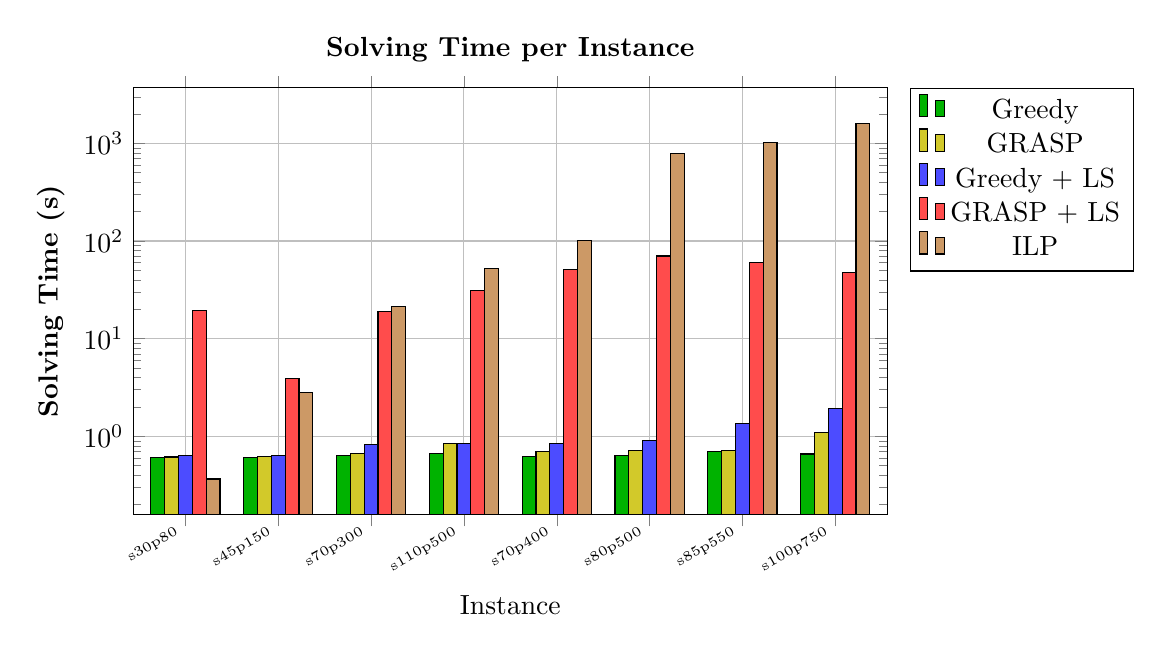
\begin{tikzpicture}
\begin{axis}[
    title={\textbf{Solving Time per Instance}},
    xlabel={Instance},
    ylabel={\textbf{Solving Time (s)}},
    grid=major,
    legend pos=outer north east,
    ybar,
    bar width=5pt,
    enlarge x limits=0.08,
    xtick={0,1,2,3,4,5,6,7},
    xticklabels={
        \tiny s30p80,
        \tiny s45p150,
        \tiny s70p300,
        \tiny s110p500,
        \tiny s70p400,
        \tiny s80p500,
        \tiny s85p550,
        \tiny s100p750
    },
    x tick label style={rotate=30, anchor=east},
    ymode=log,
    log origin=infty,
    width=0.92\textwidth,
    height=7cm,
]

% Greedy (mean_time)
\addplot[fill=green!70!black, bar shift=-10pt] coordinates {
    (0, 0.606)
    (1, 0.610)
    (2, 0.630)
    (3, 0.674)
    (4, 0.626)
    (5, 0.639)
    (6, 0.702)
    (7, 0.659)
};

% GRASP (mean_time)
\addplot[fill=yellow!80!black, bar shift=-5pt] coordinates {
    (0, 0.615)
    (1, 0.621)
    (2, 0.670)
    (3, 0.853)
    (4, 0.703)
    (5, 0.715)
    (6, 0.710)
    (7, 1.090)
};

% Greedy + LS (mean_time)
\addplot[fill=blue!70, bar shift=0pt] coordinates {
    (0, 0.630)
    (1, 0.635)
    (2, 0.821)
    (3, 0.839)
    (4, 0.841)
    (5, 0.914)
    (6, 1.351)
    (7, 1.948)
};

% GRASP + LS (mean_time)
\addplot[fill=red!70, bar shift=5pt] coordinates {
    (0, 19.453)
    (1,  3.923)
    (2, 19.094)
    (3, 30.865)
    (4, 51.376)
    (5, 70.183)
    (6, 60.897)
    (7, 47.683)
};

% ILP / CPLEX (time in seconds)
\addplot[fill=brown!80, bar shift=10pt] coordinates {
    (0,    0.366)
    (1,    2.823)
    (2,   21.169)
    (3,   52.262)
    (4,  100.356)
    (5,  791.793)
    (6, 1022.430)
    (7, 1600.768)
};

\legend{Greedy, GRASP, Greedy + LS, GRASP + LS, ILP}
\end{axis}
\end{tikzpicture}
\captionsetup{labelformat=empty}
\caption{Figure 4.2: Solving time for each algorithm across all instances (log scale).}
\label{fig:fig42}
\end{figure}


\subsubsection{Solution Quality}

\begin{figure}[H]
\centering

% % Build coordinates from individual CSV files
% \newcommand{\buildcoords}[2]{%
%     \gdef#1{}%
%     \pgfplotsforeachungrouped \i in {0,...,9} {%
%         \pgfplotstableread[col sep=comma]{data/#2/s100_p1000_instance_\i.csv}\temptable
%         \pgfplotstablegetelem{0}{mean_objective}\of\temptable
%         \ifx#1\empty
%             \xdef#1{(\i,\pgfplotsretval)}%
%         \else
%             \xdef#1{#1 (\i,\pgfplotsretval)}%
%         \fi
%     }%
% }
%
% \buildcoords{\greedydata}{s100_p1000_greedy}
% \buildcoords{\graspdata}{s100_p1000_grasp}
% \buildcoords{\greedylsdata}{s100_p1000_greedy_ls}
% \buildcoords{\grasplsdata}{s100_p1000_grasp_ls}
% \buildcoords{\cplexdata}{s100_p1000_cplex}

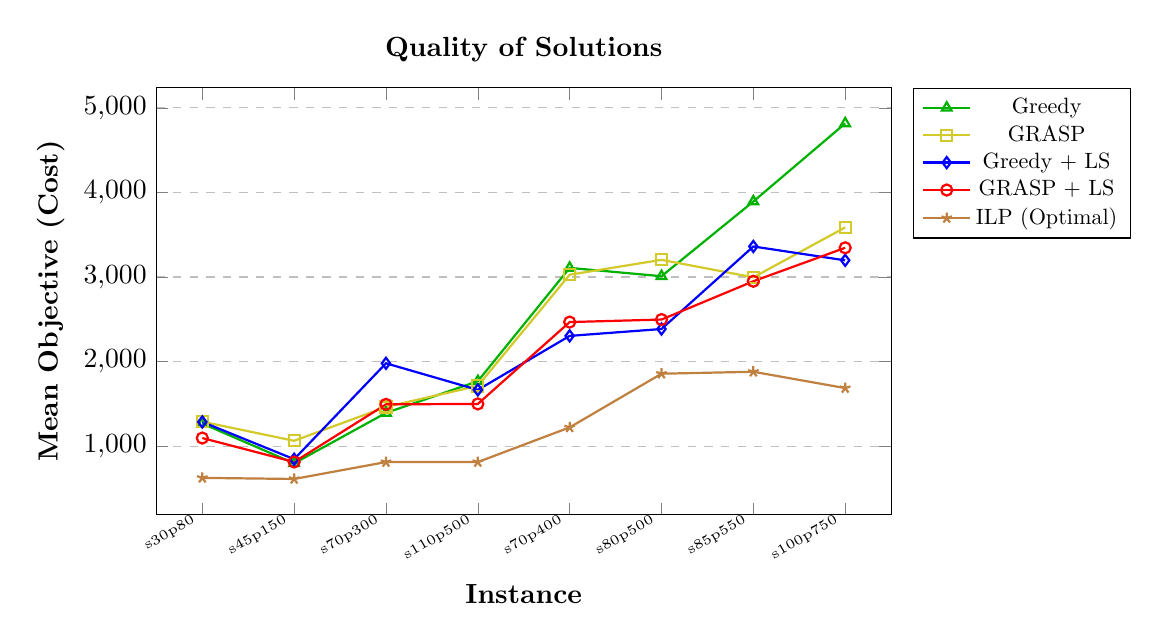
\begin{tikzpicture}
\begin{axis}[
    title={\textbf{Quality of Solutions}},
    xlabel={\textbf{Instance}},
    ylabel={\textbf{Mean Objective (Cost)}},
    xmin=-0.5, xmax=7.5,
    xtick={0,1,2,3,4,5,6,7},
    xticklabels={
        \tiny s30p80,
        \tiny s45p150,
        \tiny s70p300,
        \tiny s110p500,
        \tiny s70p400,
        \tiny s80p500,
        \tiny s85p550,
        \tiny s100p750
    },
    x tick label style={rotate=30, anchor=east},
    ymajorgrids=true,
    grid style=dashed,
    width=0.9\textwidth,
    height=7cm,
    legend pos=outer north east,
    legend style={nodes={scale=0.8, transform shape}}
]

% Greedy
\addplot[green!70!black, thick, mark=triangle] coordinates {
    (0, 1266.50)
    (1,  796.00)
    (2, 1392.20)
    (3, 1767.40)
    (4, 3107.60)
    (5, 3009.20)
    (6, 3892.80)
    (7, 4816.20)
};

% GRASP
\addplot[yellow!80!black, thick, mark=square] coordinates {
    (0, 1288.80)
    (1, 1062.50)
    (2, 1462.90)
    (3, 1711.90)
    (4, 3026.90)
    (5, 3202.80)
    (6, 2995.70)
    (7, 3586.10)
};

% Greedy + LS
\addplot[blue, thick, mark=diamond] coordinates {
    (0, 1285.70)
    (1,  845.00)
    (2, 1979.10)
    (3, 1664.70)
    (4, 2303.30)
    (5, 2384.78)
    (6, 3360.90)
    (7, 3196.80)
};

% GRASP + LS
\addplot[red, thick, mark=o] coordinates {
    (0, 1095.20)
    (1,  811.80)
    (2, 1493.70)
    (3, 1498.50)
    (4, 2466.70)
    (5, 2496.50)
    (6, 2949.40)
    (7, 3345.20)
};

% ILP (optimal)
\addplot[brown, thick, mark=star] coordinates {
    (0,  624)
    (1,  611)
    (2,  811)
    (3,  811)
    (4, 1221)
    (5, 1856)
    (6, 1879)
    (7, 1686)
};

\legend{Greedy, GRASP, Greedy + LS, GRASP + LS, ILP (Optimal)}
\end{axis}
\end{tikzpicture}
\captionsetup{labelformat=empty}
\caption{Figure 4.3: Solution Quality for each algorithm}
\label{fig:fig43}
\end{figure}



% \begin{figure}[H]
% \begin{tikzpicture}
% \begin{axis}[
%     title={\textbf{Quality of Solutions (10 datasets with 45 members)}},
%     xlabel=\textbf{{Dataset Number}},
%     ylabel=\textbf{{Total Income}},
%     xmin=1, xmax=10,
%     ymin=4000, ymax=5300,
%     xtick=data,
%     ytick={4000, 4100, 4200,4300,4400,4500,4600,4700,4800,4900,5000,5100,5200,5300},
%     ymajorgrids=true,
%     grid style=dashed,
%     width=0.7\textwidth,
%     legend pos=outer north east,
%     legend style={nodes={scale=0.8, transform shape}}
% ]

% \addplot[green,thick,mark=triangle] table {data/45members/objective_greedy.dat};
% \addplot[blue,thick,mark=triangle] table {data/45members/objective_grasp.dat};
% \addplot[brown,thick,mark=triangle] table {data/45members/objective_ls.dat};
% \addplot[black,thick,mark=triangle] table {data/45members/objective_grasp_with_ls.dat};
% \addplot[red,thick,mark=square*] table {data/45members/objective_cplex.dat};


% \legend{Greedy,GRASP(100 Iter. w/o local search  $\alpha = 0.1$),Local Search,GRASP(10 Iter. w/ local search $\alpha = 0.1$),ILP(Optimal)}

% \end{axis}
% \end{tikzpicture}
% \captionsetup{labelformat=empty}
% \caption{Figure 4.4}
% \label{fig:fig44}
% \end{figure}


% \begin{figure}[H]
% \begin{tikzpicture}
% \begin{axis}[
%     title={\textbf{Quality of Solutions (39 to 45 members)}},
%     xlabel=\textbf{{Members}},
%     ylabel=\textbf{{Total Income}},
%     xmin=39, xmax=45,
%     ymin=3500, ymax=5200,
%     xtick=data,
%     ytick={3500,3600,3700,3800,3900,4000, 4100, 4200,4300,4400,4500,4600,4700,4800,4900,5000,5100,5200},
%     ymajorgrids=true,
%     grid style=dashed,
%     width=0.7\textwidth,
%     legend pos=outer north east,
%     legend style={nodes={scale=0.8, transform shape}}
% ]

% \addplot[green,thick,mark=triangle] table {data/variable_members/objective_greedy.dat};
% \addplot[blue,thick,mark=triangle] table {data/variable_members/objective_grasp.dat};
% \addplot[brown,thick,mark=triangle] table {data/variable_members/objective_ls.dat};
% \addplot[black,thick,mark=triangle] table {data/variable_members/objective_grasp_with_ls.dat};
% \addplot[red,thick,mark=square*] table {data/variable_members/objective_cplex.dat};


% \legend{Greedy,GRASP(100 Iter. w/o local search  $\alpha = 0.1$),Local Search,GRASP(10 Iter. w/ local search $\alpha = 0.1$),ILP(Optimal)}

% \end{axis}
% \end{tikzpicture}
% \captionsetup{labelformat=empty}
% \caption{Figure 4.5}
% \label{fig:fig45}
% \end{figure}

% \nameref{fig:fig44} and \nameref{fig:fig45} shows that the Greedy approach yields the worst solution. In contrast, both GRASP (100 iterations without local search) and Local Search provide similar results. Among the heuristic methods, GRASP (10 iterations with local search) offers the best solution.

\nameref{fig:fig43} evaluates the solution quality by comparing the mean objective cost obtained by each algorithm across the instances. As this is a minimization problem, lower objective values represent superior performance.
\\
The results demonstrate a clear stratification in the quality of the solution among the tested approaches:
\begin{itemize}
    \item \textbf{Optimal Baseline:}  The exact ILP model establishes the true lower bound, consistently outperforming all heuristic methods with a mean of objective values of 1187.
    \item \textbf{Heuristic Trajectory:} The pure Greedy approach yields the worst solution quality, generating the highest cost curve across the highest instances (peaking near 4816 in Instance s100p750).Standalone GRASP seems to be a little more effective in average.
    \item \textbf{Impact of Local Search (LS):} Incorporating neighborhood search minimizes the optimality gap. GRASP + LS and the Greedy + LS variant exhibit highly competitive, intermediate performance.
    \item \textbf{Top Metaheuristic:} Ultimately, the GRASP + LS hybrid achieves the lowest average objective costs among all approximate methods (of 2016), proving to be the most effective heuristic configuration for minimizing total cost.
\end{itemize}


\subsection{Experiment Conclusion}

If the problem scale is small, we should use the exact ILP model whenever possible, as it guarantees finding the absolute optimal solution within a rational timeframe. However, for larger networks where the combinatorial explosion makes the ILP unfeasible, we need effective approximations to deliver reasonably good solutions quickly.

Among the heuristic strategies tested, the pure Greedy method is extremely fast but provides poor solution quality. Employing GRASP with local search (GRASP + LS) strikes the best balance: it significantly reduces the optimality gap and robustly achieves the lowest objective costs among our approximate methods. Therefore, for large-scale Martian network destruction scenarios, the GRASP + LS configuration stands out as the most pragmatic approach.

\section{Personal Reflections}

Initially, we had limited knowledge of advanced graph theory and were unfamiliar with concepts like minimum cuts, graph partitions, and network connectivity algorithms. We approached the algorithmic design hesitantly at first, but after receiving guidance from our professors and exploring algorithms like Stoer-Wagner and Karger's in more depth, a new mathematical world opened up for us. We were amazed by the efficiency and power of specialized graph algorithms.\\
Moreover, the optimization methods used in integer linear programming represent a significant shift in thinking. These declarative methods are incredibly elegant, and we inherently strive to pursue optimal solutions in theory. However, in practice, solving these large-scale combinatorial problems to optimality can be prohibitively costly. Consequently, we must employ heuristic and metaheuristic methods as a necessary tradeoff for scalability. It is essential to formulate, experiment, and iterate in order to discover practical solutions.\\
We will continue to refine our algorithm engineering skills, as we now firmly believe that understanding the balance between exact mathematical models and fast approximations is key to solving real-world computer science problems.


\section{Acknowledgements}

We want to give a big thank you to Prof. Enric Rodriguez and Prof. Luis Velasco for all their guidance and support throughout this report and during the whole course.

% \newpage
\appendix

% \section{Pseudocode of Auxiliary Functions for Directed Graph}


% Some auxiliary functions are utilized to process directed graphs for the \textit{Greedy}, \textit{Local Search}, and \textit{GRASP} methods.
% \begin{itemize}
%     \item The function $TopologicalSort$ implements \textbf{\textit{Kahn's algorithm}} to obtain the topological sort of a directed graph, which has $CoveredMembers$ as vertices and $Solution$ (in Greedy method, it is the partial solution) as edges. If there are edges remaining, this indicates that a cycle exists in the graph.
%     \item The function $TrimGraph$ continues to eliminate all vertices with zero indegree or zero outdegree until every remaining edge is part of a cycle.
% \end{itemize}

% \begin{algorithm}[H]
% \renewcommand{\thealgorithm}{}
% \caption{Auxiliary functions For Directed Graph}
% \begin{algorithmic}

% \Function{GetVerticesFromEdges}{$edges$}
% \State $vertices \gets \phi$
% \For{\textbf{each} $<i,j> \in edges$}
% \State $vertices \gets vertices \cup {i, j}$
% \EndFor
% \State \Return $vertices$
% \EndFunction

% \Statex

% \Function{ConstructNeighbors}{$vertices$, $eges$}
% \State $neighbors \gets \phi$
% \For{\textbf{each} $<i,j> \in edges$}
% \State $neighbors(i) \gets neighbors(i) \cup {j}$
% \EndFor
% \State \Return $neighbors$
% \EndFunction

% \Statex

% \Function{TopologicalSort}{$edges$}
% \State $topologicalOrder, indegree \gets \phi, \phi$
% \State $neighbors \gets ConstructNeighbors(vertices, edges)$
% \For{\textbf{each} $vertex \in vertices$}
%     \For{\textbf{each} $neighbor \in neighbors(vetex)$}
%         \State $indegree(neighbor) \gets indegree(neighbor) + 1$
%     \EndFor
% \EndFor
% \State $nodesWithZeroIndegree \gets \{vertex \in vertices| indegree(vertex) = 0\}$
% \While{$nodesWithZeroIndegree \neq \phi$}
%     \State $node \gets nodesWithZeroIndegree.\textrm{POP}()$
%     \State $topologicalOrder \gets topologicalOrder \cup \{node\}$
%     \For{\textbf{each} $neighbor \in neighbors(node)$}
%         \State $indegree(node) \gets indegree(node) - 1$
%         \If{$indegree(neighbor) = 0$}
%             \State $nodesWithZeroIndegree \gets nodesWithZeroIndegree \cup \{neighbor\}$
%         \EndIf
%     \EndFor
% \EndWhile
% \State \Return $topologicalOrder$
% \EndFunction

% \algstore{graph}
% \end{algorithmic}
% \end{algorithm}

% \newpage

% \begin{algorithm}
% \begin{algorithmic}
% \algrestore{graph}

% \Function{TrimGraph}{$edges$}
% \State $indegree, outdegree, previousEdges \gets \phi, \phi, \phi$
% \State $vertices \gets GetVerticesFromEdges(edges)$
% \State $neighbors \gets ConstructNeighbors(vertices, edges)$
% \For{\textbf{each} $vertex \in vertices$}
%     \State $outdegree(vertex) \gets \lvert neighbors(vertex) \rvert$
%     \For{\textbf{each} $neighbor \in neighbors(vetex)$}
%         \State $indegree(neighbor) \gets indegree(neighbor) + 1$
%     \EndFor
% \EndFor
% \State $nodesWithZeroIndegree \gets \{vertex \in vertices| indegree(vertex) = 0\}$
% \State $nodesWithZeroOutdegree \gets \{vertex \in vertices| outdegree(vertex) = 0\}$
% \While{$edges \subset previousEdges $}
% \State $previousEdges \gets edges$
% \While{$nodesWithZeroIndegree \neq \phi$}
%     \State $node \gets nodesWithZeroIndegree.\textrm{POP}()$
%     \For{\textbf{each} $neighbor \in neighbors(node)$}
%         \State $indegree(node) \gets indegree(node) - 1$
%         \State $outdegree(node) \gets outdegree(node) - 1$
%         \If{$<node, neighbor>$}
%              \State $edges.\textrm{REMOVE}(<node, neighbor>)$
%         \EndIf
%         \If{$indegree(neighbor) = 0$}
%             \State $nodesWithZeroIndegree \gets nodesWithZeroIndegree \cup \{neighbor\}$
%         \EndIf
%         \If{$outdegree(node) = 0$}
%             \State $nodesWithZeroOutdegree \gets nodesWithZeroOutdegree \cup \{node\}$
%         \EndIf
%     \EndFor
% \EndWhile
% \While{$nodesWithZeroOutdegree \neq \phi$}
%     \State $node \gets nodesWithZeroOutdegree.\textrm{POP}()$
%     \For{\textbf{each} $node' \in neighbors$}
%     \If{$outdegree(node')> 0$ AND $node \in neighbors(node')$ }
%     \State $outdegree(node') \gets outdegree(node') - 1$
%     \State $indegree(node) \gets indegree(node) - 1$
%     \If{$<node', node> \in edges$}
%         \State $edges.\textrm{REMOVE}(<node', node>)$
%     \EndIf
%     \If{$outdegree(node') = 0$}
%         \State $nodesWithZeroOutdegree \gets nodesWithZeroOutdegree \cup \{node'\}$
%     \EndIf
%     \If{$indegree(node) = 0$}
%         \State $nodesWithZeroIndegree \gets nodesWithZeroIndegree \cup \{node\}$
%     \EndIf
%     \EndIf
%     \EndFor
% \EndWhile
% \EndWhile
% \State \Return $edges, indegree, outdegree$
% \EndFunction

% \end{algorithmic}
% \end{algorithm}

\section{Source Code}

All code implementations of heuristic methods and ILP model are available at \href{https://github.com/tmactong/AMMM-project}{Github Repo}.\\
The \href{https://github.com/tmactong/AMMM-project/blob/main/README.md}{README} provides the explanation of how to use the code to solve the problem.

\end{document}